%%%%%%%%%%%%%%%%%%%%%%%%%%%%%%%%%%%%%%%%%%%%%%%%%%%%%%%%%%%%%%%%%%%%%%%%%%%%%%%
%%  LensJudge -- the human baseline for A/B/C lens grading.
%%  Standalone report (sibling of main.tex and residual.tex). Analysis code in
%%  ../parity/{fetch_vizier_paper2,intergrader_stats,grade_purity_table,
%%  human_baseline_summary,make_baseline_figures}.py; inter-team kappa in
%%  ../eval/human_ceiling.py; truth tables in ../parity/data/external/.
%%%%%%%%%%%%%%%%%%%%%%%%%%%%%%%%%%%%%%%%%%%%%%%%%%%%%%%%%%%%%%%%%%%%%%%%%%%%%%%
\documentclass[11pt,letterpaper]{article}
\usepackage{../../tech-report}
\usepackage{graphicx}

\newcommand{\lj}{\textsc{LensJudge}}
\newcommand{\qwk}{\ensuremath{\kappa_{\mathrm{qw}}}}

\title{The Human Baseline for Strong-Lens Grading:\\
       Inter-Grader Reliability and Grade-Stratified Confirmation Rates\\
       for the DESI Legacy Surveys Lens Search}
\author{Greg Benson\thanks{\texttt{benson@cs.usfca.edu}; Department of Computer
        Science, University of San Francisco, CA 94117, USA} \and
        Xiaosheng Huang\thanks{Department of Physics \& Astronomy, University of
        San Francisco; and Physics Division, Lawrence Berkeley National Laboratory}}
\date{July 2026}
\addbibresource{references.bib}

\begin{document}
\maketitle
\subtitle{What ``as good as a human grader'' must mean, measured from published data
alone: the program's first inter-grader agreement statistics, its first
confirmation-purity-per-grade table, and the concrete parity targets they set for any
machine grader}

\begin{abstract}
Any claim that an automated system grades strong-lens candidates ``at human level'' is empty
until human level is a number. For the DESI Legacy Surveys search
\citep{huang2020decals,huang2021desi,storfer2024dr9,inchausti2025} that number has never been
published: final A/B/C grades are a two-senior-grader consensus, and no paper in the series (or,
to our knowledge, in any survey's lens search) reports a chance-corrected inter-rater statistic
for expert lens grading. We recover the missing baseline from published data alone, in two
independent ways. \emph{Reliability:} the \citet{huang2021desi} VizieR catalog preserves, for
each of $1{,}312$ accepted candidates, the two graders' score average and absolute difference
--- enough to reconstruct every unordered pair of integer scores. The two graders gave the same
$1$--$4$ score on only $55.4\%$ of accepted candidates ($95\%$ CI $[52.7,58.0]$), for a
symmetrized quadratic-weighted kappa of $0.42$ $[0.37,0.47]$; on grade-A candidates --- the
search's highest-confidence class --- both graders said ``4'' only $46.5\%$ of the time, and on
$3.7\%$ of \emph{accepted} candidates one grader had voted at the reject level. Because the
catalog is truncated at acceptance, each of these is an \emph{upper} bound on full-pool
agreement. Against independent expert teams grading the same candidates the ceiling is lower
still ($\qwk=0.29$ vs.\ the SuGOHI committee, $n=103$; $0.17$ vs.\ the Euclid Q1 panel,
$n=24$). \emph{Validity:} assembling every published per-target follow-up outcome for the
program's candidates --- HST SNAP \citep{huang2025foundry1}, DESI EDR spectroscopy
\citep{huang2025foundry2}, Keck/NIRES \citep{agarwal2025foundry3}, VLT/MUSE
\citep{lin2025foundry4}, AGEL \citep{tran2022agel,barone2025agel}, HSC$\times$DESI
\citep{shu2025hscdesi}, and SuGOHI spectroscopy \citep{sonnenfeld2018sugohi} --- yields the
program's first grade-stratified confirmation table: of $162$ followed-up graded candidates,
$130$ are decided, with purity $79/83=95.2\%$ $[88.9,98.4]$ for grade A, $23/25=92.0\%$ for B,
and $20/22=90.9\%$ for C --- statistically indistinguishable across grades on this (curated,
best-first) follow-up mix, and pointedly \emph{not} $100\%$ for grade A: four grade-A candidates
are spectroscopically refuted, all arcs at the wrong or same redshift. Together these results
replace ``trained humans reliably assign A/B grades'' with measured quantities, and they define
the two pre-registrable targets any machine grader must meet: an agreement target (match one
grader's $\qwk$ against the consensus, bounded by $[0.29,\,0.78]$) and a truth target
(non-inferior confirmed-vs-refuted discrimination on the same follow-up set). The machinery and
caveats for both are laid out here.
\end{abstract}

\section{Why a human baseline}\label{sec:why}
The DESI Legacy Surveys strong-lens search grades neural-network recommendations by expert
visual inspection: candidates surviving a probability cut are scored by team members and
published with grades A (``high level of confidence''), B, or C. Downstream uses --- follow-up
target selection, purity claims, training labels for the next finder, and any assessment of an
automated grader such as \lj{} --- treat the grade as a stable quantity. Part~I of the \lj{}
report measured how well an automated grader reproduces the consensus grade at DESI resolution
and found $\kappa\approx0$; but it also found that \emph{independent expert teams} agree with
the DESI consensus only at $\qwk\approx0.3$, and the literature reports high intra-expert
inconsistency in every controlled experiment \citep{rojas2023vi,canameras2021holismokes,
petrillo2019links,euclidq1engine}. What has been missing is the number for \emph{this} program's
own graders: no inter-grader agreement statistic and no confirmation rate conditioned on grade
has ever been published, here or (to our knowledge) for any survey's expert lens grading. This
report supplies both, from published data alone, with no new grading campaign.

Two distinct questions hide inside ``as good as a human'': \emph{reliability} (do graders agree
with each other?) and \emph{validity} (do the grades predict what spectroscopy and
high-resolution imaging later decide?). We measure both, because they set different machine
targets: a machine can only be asked to agree with the consensus as well as a human does
(\S\ref{sec:reliability}--\ref{sec:crossteam}), and it can be asked to discriminate real from
false candidates at least as well as the grades do (\S\ref{sec:purity}).

\section{The recovered two-grader data}\label{sec:data}
In \citet{huang2021desi} (``Paper~II''), two graders each assigned an integer score $1$--$4$
to every candidate surviving triage; the published catalog records the pair's \emph{average}
(\texttt{Score} $\in[2.0,4.0]$, since only averages $\geq2.0$ were accepted) and, crucially, the
\emph{absolute difference} (\texttt{delSc} $\in\{0,1,2\}$) --- columns preserved in the VizieR
table \texttt{J/ApJ/909/27/cand} but absent from every other release of the series. The
unordered pair of integer scores is exactly $\{\texttt{Score}-\texttt{delSc}/2,\,
\texttt{Score}+\texttt{delSc}/2\}$; grader \emph{identity} is lost, so all statistics below
treat the raters as interchangeable. Parity of $2\times\texttt{Score}$ and \texttt{delSc}
validates the reconstruction row by row: $1{,}310$ of $1{,}312$ rows are consistent with two
integer scores (the two exceptions, DESI-094.5639$+$50.3059 and DESI-227.9362$+$06.5090, carry
impossible combinations --- data-entry glitches --- and are excluded).

Letter grades follow from the average (A: $\geq3.5$; B: $3.0$; C: $2.0$--$2.5$), which checks
out exactly against the published counts ($216$~A $=100$ pairs of $\{4,4\}$ $+115$ of $\{3,4\}$
$+1$ glitch; $199$~B; $897$~C). Figure~\ref{fig:pairs} shows the full joint distribution.

\begin{figure}[t]
  \centering
  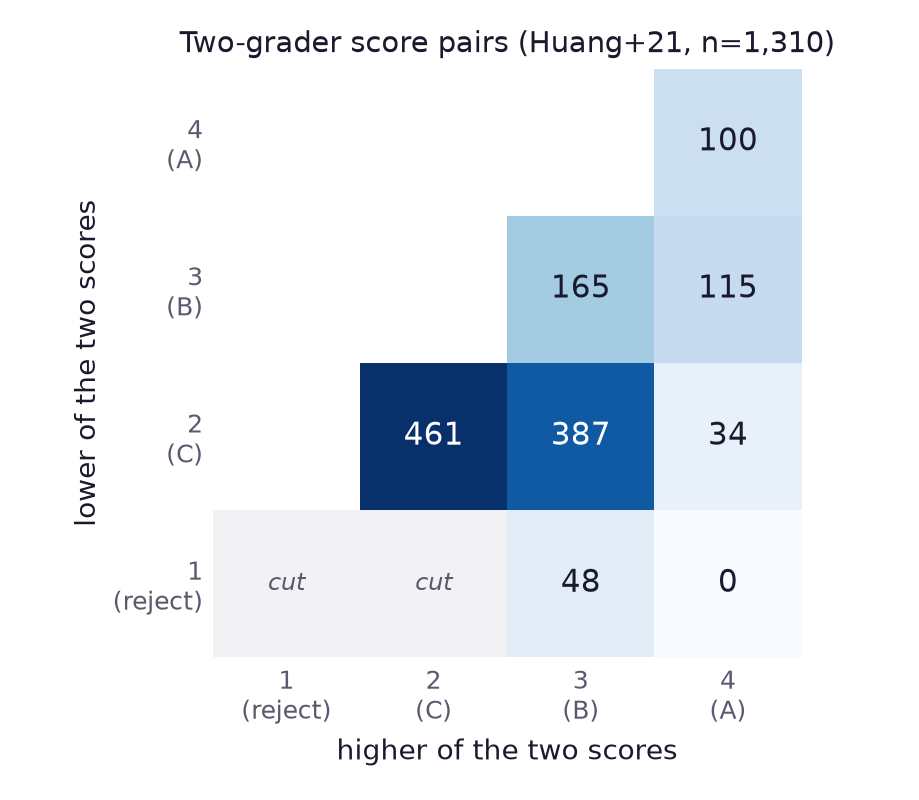
\includegraphics[width=0.62\linewidth]{figures/baseline_pair_heatmap.png}
  \caption{The two graders' unordered score pairs for all $1{,}310$ reconstructable accepted
  candidates in \citet{huang2021desi}. Cells marked \emph{cut} cannot appear in the published
  catalog (pairs averaging below $2.0$ were not accepted), which is why every statistic in
  \S\ref{sec:reliability} is an upper bound on full-pool agreement. Note the $48$ candidates
  scored $\{1,3\}$: one grader at reject level, the other at grade-B confidence, on the same
  cutout.}\label{fig:pairs}
\end{figure}

\section{Inter-grader reliability}\label{sec:reliability}
Table~\ref{tab:reliability} gives the program's first inter-grader agreement statistics
($2{,}000$-sample bootstrap over candidates, seed $2026$). Three facts carry the story:

\begin{itemize}
\item \textbf{Exact agreement is a coin flip plus a little.} The two graders gave the same
integer score on $55.4\%$ of accepted candidates; $38.3\%$ differ by one step and $6.3\%$ by
two. The symmetrized quadratic-weighted kappa is $0.42$ (``moderate''), identical to
Krippendorff's interval $\alpha$ as expected for two coders. For comparison, \citet{rojas2023vi}
measured $73\%$ \emph{intra}-rater repeat consistency --- an individual agrees with the same
image shown twice more often than these two experts agree with each other.
\item \textbf{The top grade is the least internally stable.} Within published grade A, both
graders voted ``4'' only $46.5\%$ $[40.2,53.2]$ of the time; the majority of A's are a
$\{3,4\}$ split. (Grade B's higher within-grade agreement, $82.9\%$, is partly mechanical: a
$\{3,4\}$ pair averages to A and a $\{2,3\}$ pair to C, so B can only arise as $\{3,3\}$ or the
rare $\{2,4\}$.)
\item \textbf{Acceptance can hinge on one vote.} $3.7\%$ of \emph{accepted} candidates ($48$ of
$1{,}310$) carry a $\{1,3\}$ pair --- one grader would have rejected outright. And the
truncation cut means every pair in which \emph{both} graders were low is invisible: these
numbers are ceilings.
\end{itemize}

\begin{table}[t]
\centering\small
\begin{tabular}{lcc}
\hline
statistic (Paper II, $n=1{,}310$ accepted candidates) & value & $95\%$ CI \\
\hline
exact score agreement $P(\texttt{delSc}=0)$            & $0.554$ & $[0.527, 0.580]$ \\
one-step disagreement                                  & $0.383$ & $[0.357, 0.411]$ \\
two-step disagreement                                  & $0.063$ & $[0.050, 0.076]$ \\
one grader at reject level (among accepted)            & $0.037$ & $[0.026, 0.047]$ \\
symmetrized \qwk{} (scores $1$--$4$)                   & $0.420$ & $[0.371, 0.468]$ \\
Krippendorff $\alpha$ (interval)                       & $0.420$ & $[0.371, 0.468]$ \\
individual grader vs.\ published consensus \qwk{}      & $0.776$ & $[0.757, 0.793]$ \\
\quad (upper bound: each grader is half the consensus) & & \\
both graders ``4'' within grade A                      & $0.465$ & $[0.402, 0.532]$ \\
exact agreement within grade B                         & $0.829$ & $[0.776, 0.881]$ \\
exact agreement within grade C                         & $0.515$ & $[0.480, 0.547]$ \\
\hline
\end{tabular}
\caption{Inter-grader reliability reconstructed from the \citet{huang2021desi} VizieR
\texttt{Score}/\texttt{delSc} columns. All quantities are upper bounds on full-pool agreement
(truncation at acceptance). Code: \texttt{parity/intergrader\_stats.py}.}\label{tab:reliability}
\end{table}

The last row block of Table~\ref{tab:reliability} contains the number a machine should be
scored against for an \emph{agreement} claim: an individual trained grader matches the
published consensus at $\qwk=0.776$ $[0.757,0.793]$ --- and even this is inflated, since each
grader contributes half of that consensus. A machine that reaches
$\qwk\approx0.78$ against the published grades is \emph{indistinguishable from a member of the
grading team}; one that reaches the two graders' mutual $0.42$ already agrees with a Huang-group
grader as well as the two graders agree with each other.

\section{Independent teams agree far less}\label{sec:crossteam}
The Paper~II pair shares a rubric, a rendering, and a screen. Independent expert teams grading
the \emph{same} candidates under their own protocols set a lower --- and for machine-parity
purposes, arguably fairer --- ceiling. Re-deriving the \lj{} Part~I crossmatch from its now
fully staged inputs reproduces: DESI consensus vs.\ the SuGOHI $\sim$9-grader committee
\citep{sonnenfeld2018sugohi}, $\qwk = 0.288$ $[0.121, 0.444]$, $n=103$, exact agreement
$38.8\%$; DESI vs.\ the Euclid Q1 $\sim$10-expert panel \citep{euclidq1engine},
$\qwk = 0.165$, $n=24$. The literature concurs: only $30\%$ of a HOLISMOKES blind set had zero
score dispersion among five graders \citep{canameras2021holismokes}; only $25.8\%$ of another
team's grade-A DR9 candidates received A or B from this program's graders
\citep{storfer2024dr9}; the Euclid Q1 panel is decisive on only $\sim$$38\%$ of its candidates
\citep{euclidq1engine}; and all eleven confirmed SLACS lenses embedded in DES-quality imaging
were collectively judged non-lenses by $55$ experts \citep{rojas2023vi}.

\section{Grade-stratified confirmation rates}\label{sec:purity}
Reliability is not validity: graders could disagree yet still, in aggregate, select real
lenses. We therefore assembled every published per-target follow-up outcome for the program's
candidates into normalized truth tables --- $551$ targets across seven campaigns --- and
cross-matched them (radius $2''$) against the unified graded-candidate table ($4{,}354$ unique
candidates from \citealt{huang2020decals,huang2021desi,storfer2024dr9,inchausti2025}). Each
matched candidate gets one outcome by precedence (confirmed $>$ refuted $>$ lens-$z$-only $>$
inconclusive $>$ pending); no candidate is both confirmed and refuted by different campaigns.
Table~\ref{tab:purity} and Figure~\ref{fig:purity} give the result: $162$ unique graded
candidates have follow-up, $130$ are decided, and confirmation purity among the decided is
$95.2\%$ (A), $92.0\%$ (B), $90.9\%$ (C) --- high everywhere, flat in grade within the errors.

\begin{table}[t]
\centering\small
\begin{tabular}{lrrrrrrl}
\hline
grade & followed & confirmed & refuted & lens-$z$ only & pend./inc. & decided & purity (Jeffreys $95\%$) \\
\hline
A & $99$ & $79$ & $4$ & $10$ & $6$ & $83$ & $0.952$ $[0.889, 0.984]$ \\
B & $30$ & $23$ & $2$ & $4$  & $1$ & $25$ & $0.920$ $[0.767, 0.983]$ \\
C & $33$ & $20$ & $2$ & $7$  & $4$ & $22$ & $0.909$ $[0.739, 0.981]$ \\
\hline
\end{tabular}
\caption{The program's first confirmation-rate-per-grade table, over all published follow-up
(Foundry I--IV, AGEL DR2, HSC$\times$DESI, SuGOHI spectroscopy). ``Decided'' $=$ confirmed $+$
refuted. Follow-up targets were curated --- mostly best-first --- so purities are upper bounds
and the grade comparison inherits each campaign's selection function
(\S\ref{sec:caveats}).}\label{tab:purity}
\end{table}

\begin{figure}[t]
  \centering
  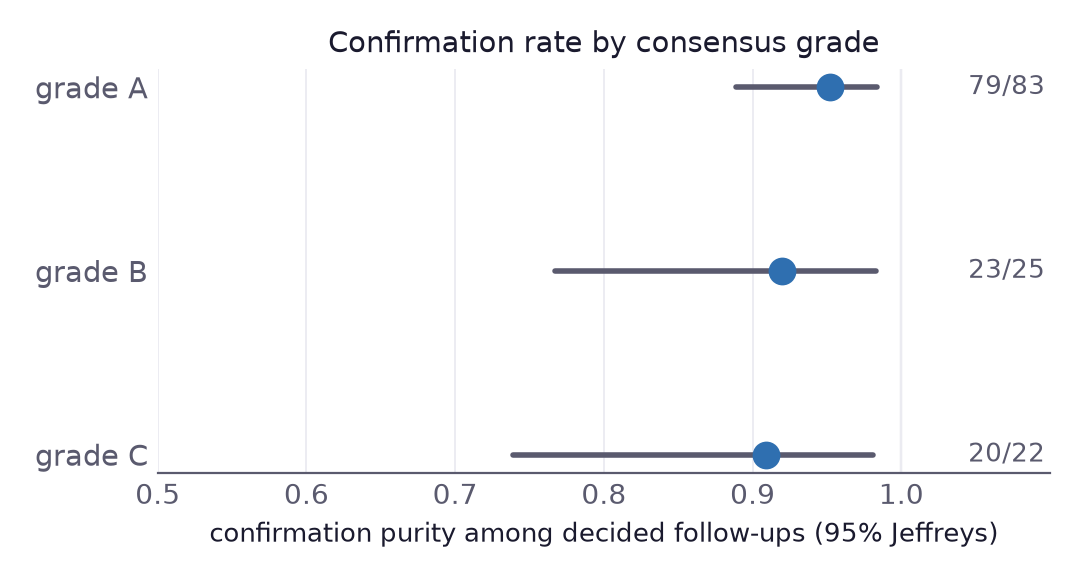
\includegraphics[width=0.75\linewidth]{figures/baseline_purity.png}
  \caption{Confirmation purity by consensus grade among decided follow-ups, with $95\%$
  Jeffreys intervals. The three grades are statistically indistinguishable on this follow-up
  mix.}\label{fig:purity}
\end{figure}

Two readings matter. First, \textbf{grade A is not infallible}: four grade-A candidates are
spectroscopically refuted by VLT/MUSE \citep{lin2025foundry4} --- a spiral arm at the galaxy's
own redshift, a tidal tail between merging galaxies at one redshift, a blue arc at exactly the
deflector's redshift, and an ``arc'' that is a \emph{foreground} object. Every one is the
morphology-only failure mode: an arc-shaped feature whose redshift, not its shape, is
disqualifying. Grades assigned from $1.3''$-seeing pixels cannot see redshift. Second,
\textbf{grade C is not mostly junk} --- $20$ of $22$ decided C's are real lenses. This
complements the Part~I Euclid result ($53\%$ of DESI grade-C candidates re-grade to A/B at
$0.1''$): C tracks \emph{resolution-limited visibility}, not lens likelihood, on the pool that
teams chose to follow up.

For completeness: the six AGEL false positives \citep{barone2025agel} all trace to
DES/Jacobs-selected candidates --- none lies within arcminutes of any candidate in this
program's catalogs --- and Foundry~II's grade-agnostic DESI Secondary Target Program ($2{,}157$
systems) remains the future, selection-clean version of Table~\ref{tab:purity}
\citep{huang2025foundry2}.

\section{The machine-parity targets these results set}\label{sec:targets}
These measurements convert ``performs as well as human experts'' into two falsifiable,
pre-registrable endpoints for any automated grader of DESI-resolution cutouts:

\begin{description}
\item[E1 --- agreement parity.] Score the machine's grades against the published consensus with
\qwk{}. The human anchors are now measured: $0.776$ (an individual team grader, upper bound),
$0.42$ (the two graders' mutual agreement), $0.29$ (an independent expert team). A defensible
claim of agreement-parity is $\qwk \geq 0.29$ with a CI excluding $0$ (matches an independent
expert team); a strong claim is $\qwk$ compatible with $0.776$ (indistinguishable from a team
member). \lj{} Part~I's DESI-resolution graders sat at $\kappa\approx0$ --- the gap to close is
now quantified.
\item[E2 --- truth parity.] On candidates with decided follow-up, compare machine score and
human grade (as an ordinal score) as paired predictors of confirmed-vs-refuted, via
non-inferiority on AUC with a pre-registered margin. The human operating points from
Table~\ref{tab:purity} --- e.g.\ A/B selection at $\sim$$94\%$ decided purity on the curated mix
--- are the benchmarks. Today's decided sample ($n=130$, only $8$ refutations) supports
estimation but is thin for a verdict at small margins; the forthcoming grade-agnostic Foundry
program and the Euclid Q1/DR1 truth sets (hundreds of space-resolution adjudications inside the
Legacy footprint) are what will power it properly.
\end{description}

Both endpoints need the machine to be given the graders' actual task: Paper~II--DR10 graders saw
multi-band composites with viewer context and redshift metadata, not bare $101$-px pixels ---
an input asymmetry any fair comparison must remove.

\section{Caveats}\label{sec:caveats}
(i)~Truncation: the Paper~II pairs exist only for accepted candidates; all reliability numbers
are upper bounds. (ii)~Rater anonymity: unordered pairs support interchangeable-rater statistics
only; per-grader bias is unrecoverable. (iii)~Selection: follow-up campaigns targeted their best
candidates (Foundry~I explicitly so, and its $51/51$ confirmation rate should be read as a
property of that curation); purities are upper bounds and cross-grade comparisons inherit the
selection. (iv)~Truth precedence: ``confirmed'' requires both lens and source redshifts (or HST
morphology per Foundry~I); source-only AGEL systems are held out as inconclusive. (v)~The
cross-team \qwk{} compares different rubrics, renderings, and (for Euclid) resolutions; part of
that gap is real information difference, so the same-regime SuGOHI comparison is the cleaner
anchor. (vi)~One grading pass per pair: intra-rater noise (Rojas's $73\%$) is not separable from
inter-rater disagreement here.

\section{Reproducibility}\label{sec:repro}
All inputs are published catalogs. \texttt{parity/fetch\_vizier\_paper2.py} retrieves and
validates the Paper~II table (row parity check; $100\%$ join against the local reproduction
catalog); \texttt{parity/intergrader\_stats.py} computes Table~\ref{tab:reliability};
\texttt{eval/crossmatch\_external.py} rebuilds the master candidate table and the
SuGOHI/Euclid crossmatches ($104$ and $24$ matches, reproducing Part~I);
\texttt{eval/human\_ceiling.py} computes the cross-team \qwk{};
\texttt{parity/data/external/*.csv} hold the seven normalized per-target truth tables (each
machine-parsed from the papers' own LaTeX/VizieR/Zenodo sources, with per-row provenance);
\texttt{parity/grade\_purity\_table.py} produces Table~\ref{tab:purity}; and
\texttt{parity/human\_baseline\_summary.py} assembles the combined baseline table. Figures:
\texttt{parity/make\_baseline\_figures.py}.

\bibliographystyle{plainnat}
\bibliography{references}

\end{document}
